\section{平面与直线}

\begin{problem}{平面位置及其方程特点}{Plane-Position-Features}
    指出下列平面位置的特点，并作图.
    \begin{enumerate}
        \item $2x + 2y + 2z = -1$;
        \item $3x - 3y + 2 = 0$;
        \item $y - 3z = 0$;
        \item $3x - 2 = 0$.
    \end{enumerate}
\end{problem}

\begin{solution}

    \ansitem{1}

    将平面方程 $2x + 2y + 2z = -1$ 改写为截距式方程：
    \begin{equation}
        \frac{x}{-\frac{1}{2}} + \frac{y}{-\frac{1}{2}} + \frac{z}{-\frac{1}{2}} = 1
    \end{equation}
    可知该平面在 $x$ 轴、$y$ 轴、$z$ 轴上的截距均为 $-\frac{1}{2}$．由于方程中包含 $x, y, z$ 三个变量，且常数项不为零，故该平面与三个坐标轴均相交，且不过原点．
    \begin{equation}
        \boxed{\text{该平面与三个坐标轴均相交，且不过原点}}
    \end{equation}

    \begin{center}
        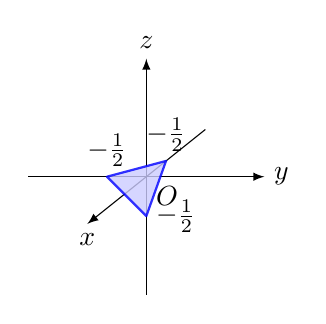
\begin{tikzpicture}[x={(-0.5cm,-0.4cm)}, y={(1cm,0cm)}, z={(0cm,1cm)}, >=latex]
            \draw[->] (-1.5,0,0) -- (1.5,0,0) node[below] {$x$};
            \draw[->] (0,-1.5,0) -- (0,1.5,0) node[right] {$y$};
            \draw[->] (0,0,-1.5) -- (0,0,1.5) node[above] {$z$};
            \node[below right] at (0,0,0) {$O$};

            \filldraw[fill=blue!20, opacity=0.8, draw=blue, thick, join=round]
            (-0.5,0,0) -- (0,-0.5,0) -- (0,0,-0.5) -- cycle;

            \node[above] at (-0.5,0,0) {$-\frac{1}{2}$};
            \node[above] at (0,-0.5,0) {$-\frac{1}{2}$};
            \node[right] at (0,0,-0.5) {$-\frac{1}{2}$};
        \end{tikzpicture}
    \end{center}

    \ansitem{2}

    由平面方程 $3x - 3y + 2 = 0$ 可知，方程中不含变量 $z$．其法向量为 $\symbfit{n} = (3, -3, 0)$，满足 $\symbfit{n} \cdot \symbfit{k} = 0$，其中 $\symbfit{k} = (0, 0, 1)$ 为 $z$ 轴的方向向量．

    这表明该平面的法向量垂直于 $z$ 轴，从而平面平行于 $z$ 轴．同时常数项不为零，故平面不包含 $z$ 轴（即不过原点）．它在 $xOy$ 面上的交线方程为 $y = x + \frac{2}{3}$．
    \begin{equation}
        \boxed{\text{该平面平行于 } z \text{ 轴，且不过原点}}
    \end{equation}

    \begin{center}
        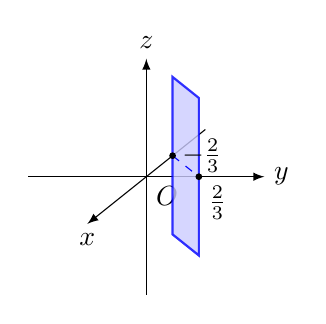
\begin{tikzpicture}[x={(-0.5cm,-0.4cm)}, y={(1cm,0cm)}, z={(0cm,1cm)}, >=latex]
            \draw[->] (-1.5,0,0) -- (1.5,0,0) node[below] {$x$};
            \draw[->] (0,-1.5,0) -- (0,1.5,0) node[right] {$y$};
            \draw[->] (0,0,-1.5) -- (0,0,1.5) node[above] {$z$};
            \node[below right] at (0,0,0) {$O$};

            \filldraw[fill=blue!20, opacity=0.8, draw=blue, thick]
            (-0.667, 0, -1) -- (0, 0.667, -1) -- (0, 0.667, 1) -- (-0.667, 0, 1) -- cycle;
            \draw[dashed, blue] (-0.667, 0, 0) -- (0, 0.667, 0);
            \node[right] at (-0.667, 0, 0) {$-\frac{2}{3}$};
            \node[below right] at (0, 0.667, 0) {$\frac{2}{3}$};
            \draw[fill=black] (-0.667,0,0) circle (1pt);
            \draw[fill=black] (0,0.667,0) circle (1pt);
        \end{tikzpicture}
    \end{center}

    \ansitem{3}

    由平面方程 $y - 3z = 0$ 可知，方程中不含变量 $x$，且常数项为零．

    不含变量 $x$ 意味着其法向量 $\symbfit{n} = (0, 1, -3)$ 垂直于 $x$ 轴的方向向量 $\symbfit{i} = (1, 0, 0)$，即平面平行于 $x$ 轴；常数项为零意味着平面经过原点．平行于 $x$ 轴且经过原点的平面必然包含 $x$ 轴．它在 $yOz$ 面上的交线方程为 $y = 3z$．
    \begin{equation}
        \boxed{\text{该平面过原点，且包含 } x \text{ 轴}}
    \end{equation}

    \begin{center}
        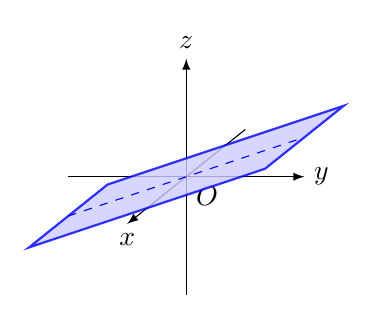
\begin{tikzpicture}[x={(-0.5cm,-0.4cm)}, y={(1cm,0cm)}, z={(0cm,1cm)}, >=latex]
            \draw[->] (-1.5,0,0) -- (1.5,0,0) node[below] {$x$};
            \draw[->] (0,-1.5,0) -- (0,1.5,0) node[right] {$y$};
            \draw[->] (0,0,-1.5) -- (0,0,1.5) node[above] {$z$};
            \node[below right] at (0,0,0) {$O$};

            \filldraw[fill=blue!20, opacity=0.8, draw=blue, thick]
            (1, -1.5, -0.5) -- (1, 1.5, 0.5) -- (-1, 1.5, 0.5) -- (-1, -1.5, -0.5) -- cycle;
            \draw[dashed, blue] (0, -1.5, -0.5) -- (0, 1.5, 0.5);
        \end{tikzpicture}
    \end{center}

    \ansitem{4}

    由平面方程 $3x - 2 = 0$ 可知，方程中不含变量 $y$ 和 $z$，可化简为 $x = \frac{2}{3}$．

    其法向量为 $\symbfit{n} = (3, 0, 0)$，由于 $\symbfit{n}$ 平行于 $x$ 轴的方向向量 $\symbfit{i} = (1, 0, 0)$，表明该平面垂直于 $x$ 轴，从而平行于 $yOz$ 坐标面．它在 $x$ 轴上的截距为 $\frac{2}{3}$．
    \begin{equation}
        \boxed{\text{该平面平行于 } yOz \text{ 坐标面}}
    \end{equation}

    \begin{center}
        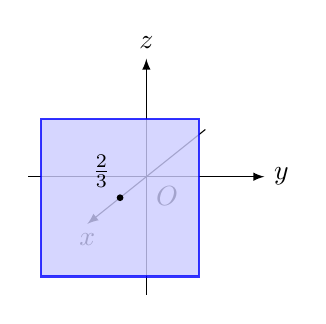
\begin{tikzpicture}[x={(-0.5cm,-0.4cm)}, y={(1cm,0cm)}, z={(0cm,1cm)}, >=latex]
            \draw[->] (-1.5,0,0) -- (1.5,0,0) node[below] {$x$};
            \draw[->] (0,-1.5,0) -- (0,1.5,0) node[right] {$y$};
            \draw[->] (0,0,-1.5) -- (0,0,1.5) node[above] {$z$};
            \node[below right] at (0,0,0) {$O$};

            \filldraw[fill=blue!20, opacity=0.8, draw=blue, thick]
            (0.667, -1, -1) -- (0.667, 1, -1) -- (0.667, 1, 1) -- (0.667, -1, 1) -- cycle;

            \node[above left] at (0.667, 0, 0) {$\frac{2}{3}$};
            \draw[fill=black] (0.667,0,0) circle (1pt);
        \end{tikzpicture}
    \end{center}

\end{solution}


\begin{problem}{平面方程}{Plane-Equation}
    试求通过点 $M_1(2, -1, 3)$ 和 $M_2(3, 1, 2)$ 且平行于向量 $\symbfit{v} = (3, -1, 4)$ 的平面方程.
\end{problem}

\begin{solution}
    首先计算向量 $\overrightarrow{M_1 M_2}$：
    \begin{equation}
        \overrightarrow{M_1 M_2} = (3-2, 1-(-1), 2-3) = (1, 2, -1)
    \end{equation}
    由于所求平面平行于 $\symbfit{v}$ 且包含直线 $M_1 M_2$，故平面的法向量 $\symbfit{n}$ 可取为：
    \begin{equation}
        \symbfit{n} = \overrightarrow{M_1 M_2} \times \symbfit{v} = \begin{bmatrix} \symbfit{i} & \symbfit{j} & \symbfit{k} \\ 1 & 2 & -1 \\ 3 & -1 & 4 \end{bmatrix} = 7\symbfit{i} - 7\symbfit{j} - 7\symbfit{k}
    \end{equation}
    取简化后的法向量 $\symbfit{n}' = (1, -1, -1)$，利用点法式方程，过点 $M_1(2, -1, 3)$：
    \begin{equation}
        1(x - 2) - 1(y + 1) - 1(z - 3) = 0 \implies x - y - z = 0
    \end{equation}
    因此，所求平面方程为：
    \begin{equation}
        \boxed{x - y - z = 0}
    \end{equation}
\end{solution}

\begin{problem}{平面的截距式方程}{Intercept-Form}
    设平面通过点 $(5, -7, 4)$ 且在 $x, y, z$ 三轴上的截距相等，求平面方程.
\end{problem}

\begin{solution}
    若截距 $a \neq 0$，设平面方程为截距式：
    \begin{equation}
        \frac{x}{a} + \frac{y}{a} + \frac{z}{a} = 1 \implies x + y + z = a
    \end{equation}
    将点 $(5, -7, 4)$ 代入方程：
    \begin{equation}
        5 - 7 + 4 = a \implies a = 2
    \end{equation}
    此时平面方程为 $x + y + z - 2 = 0$．若截距 $a = 0$，则平面通过原点，设方程为 $Ax + By + Cz = 0$，由截距相等且过点 $(5, -7, 4)$ 知，此类平面不唯一，通常按非零截距处理．综上所得：
    \begin{equation}
        \boxed{x + y + z - 2 = 0}
    \end{equation}
\end{solution}

\begin{problem}{平面位置关系判断}{Plane-Relationship}
    试判断下列方程组中各组平面的位置关系（平行, 重合, 相交, 垂直）.
    \begin{enumerate}
        \item $2x - 3y + 5z - 7 = 0$ 与 $2x - 3y + 5z + 3 = 0$；
        \item $4x + 2y - 4z + 5 = 0$ 与 $2x + y + 2z - 1 = 0$；
        \item $x - 3z + 2 = 0$ 与 $2x - 6z + 4 = 0$；
        \item $3x - y - 2z - 5 = 0$ 与 $x + 9y - 3z + 2 = 0$.
    \end{enumerate}
\end{problem}

\begin{solution}
    \ansitem{1} 平行

    两平面的法向量分别为 $\symbfit{n}_1 = (2, -3, 5)$，$\symbfit{n}_2 = (2, -3, 5)$．
    \begin{equation}
        \text{因为} \quad \frac{2}{2} = \frac{-3}{-3} = \frac{5}{5} \neq \frac{-7}{3}
    \end{equation}
    故两平面平行．
    \begin{equation}
        \boxed{\text{平行}}
    \end{equation}

    \ansitem{2} 相交

    两平面的法向量分别为 $\symbfit{n}_1 = (4, 2, -4)$，$\symbfit{n}_2 = (2, 1, 2)$．
    \begin{equation}
        \text{因为} \quad \frac{4}{2} = \frac{2}{1} \neq \frac{-4}{2} \quad \text{且} \quad \symbfit{n}_1 \cdot \symbfit{n}_2 = 8 + 2 - 8 = 2 \neq 0
    \end{equation}
    故两平面相交但不垂直．
    \begin{equation}
        \boxed{\text{相交}}
    \end{equation}

    \ansitem{3} 重合

    两平面的方程分别为 $\Pi_1: x - 3z + 2 = 0$ 与 $\Pi_2: 2x - 6z + 4 = 0$．
    \begin{equation}
        \text{观察得} \quad \Pi_2 = 2 \Pi_1
    \end{equation}
    对应系数成比例且常数项亦成比例，故两平面重合．
    \begin{equation}
        \boxed{\text{重合}}
    \end{equation}

    \ansitem{4} 垂直

    两平面的法向量分别为 $\symbfit{n}_1 = (3, -1, -2)$，$\symbfit{n}_2 = (1, 9, -3)$．计算其点积：
    \begin{equation}
        \symbfit{n}_1 \cdot \symbfit{n}_2 = 3 \times 1 + (-1) \times 9 + (-2) \times (-3) = 3 - 9 + 6 = 0
    \end{equation}
    由于法向量垂直，故两平面垂直．
    \begin{equation}
        \boxed{\text{垂直}}
    \end{equation}
\end{solution}


\begin{problem}{平面方程}{Plane-Equation-2}
    求通过点 $M(3, -1, 1)$ 且同时垂直于两个平面 $2x - z + 1 = 0$ 和 $y = 0$ 的平面方程.
\end{problem}

\begin{solution}
    已知两平面的法向量分别为 $\symbfit{n}_1 = (2, 0, -1)$ 与 $\symbfit{n}_2 = (0, 1, 0)$. 设所求平面的法向量为 $\symbfit{n}$, 则有
    \begin{equation}
        \symbfit{n} = \symbfit{n}_1 \times \symbfit{n}_2 = \begin{vmatrix} \symbfit{i} & \symbfit{j} & \symbfit{k} \\ 2 & 0 & -1 \\ 0 & 1 & 0 \end{vmatrix} = (1, 0, 2)
    \end{equation}
    利用点法式方程, 该平面通过点 $M(3, -1, 1)$, 则有
    \begin{equation}
        \begin{aligned}
                     & 1(x - 3) + 0(y + 1) + 2(z - 1) = 0 \\
            \implies & x + 2z - 5 = 0
        \end{aligned}
    \end{equation}
    故所求平面方程为
    \begin{equation}
        \boxed{x + 2z - 5 = 0}
    \end{equation}
\end{solution}

\begin{problem}{平行平面}{Parallel-Plane}
    求通过点 $M(-5, 2, -1)$ 且平行于坐标面 $Oyz$ 的平面的方程.
\end{problem}

\begin{solution}
    由于坐标面 $Oyz$ 的方程为 $x = 0$, 其法向量为 $\symbfit{n} = (1, 0, 0)$. 所求平面与其平行, 故可设所求平面方程为 $x + D = 0$. 将点 $M(-5, 2, -1)$ 代入得
    \begin{equation}
        -5 + D = 0 \implies D = 5
    \end{equation}
    因此所求平面方程为
    \begin{equation}
        \boxed{x + 5 = 0}
    \end{equation}
\end{solution}

\begin{problem}{平面夹角}{Angle-Between-Planes}
    求下列各对平面的夹角：
    \begin{enumerate}
        \item $2x - y + z - 7 = 0$ 和 $x + y + 2z - 11 = 0$;
        \item $4x + 2y + 4z - 7 = 0$ 和 $3x - 4y = 0$.
    \end{enumerate}
\end{problem}

\begin{solution}
    \ansitem{1}
    设两平面的法向量分别为 $\symbfit{n}_1 = (2, -1, 1)$ 和 $\symbfit{n}_2 = (1, 1, 2)$. 设两平面夹角为 $\theta$, 则
    \begin{equation}
        \cos \theta = \frac{|\symbfit{n}_1 \cdot \symbfit{n}_2|}{|\symbfit{n}_1||\symbfit{n}_2|} = \frac{|2 \cdot 1 + (-1) \cdot 1 + 1 \cdot 2|}{\sqrt{2^2 + (-1)^2 + 1^2} \cdot \sqrt{1^2 + 1^2 + 2^2}} = \frac{3}{\sqrt{6} \cdot \sqrt{6}} = \frac{1}{2}
    \end{equation}
    由于 $\theta \in [0, \uppi/2]$, 故
    \begin{equation}
        \boxed{\theta = \frac{\uppi}{3}}
    \end{equation}

    \ansitem{2}
    设两平面的法向量分别为 $\symbfit{n}_1 = (4, 2, 4)$ 和 $\symbfit{n}_2 = (3, -4, 0)$. 设两平面夹角为 $\theta$, 则
    \begin{equation}
        \cos \theta = \frac{|\symbfit{n}_1 \cdot \symbfit{n}_2|}{|\symbfit{n}_1||\symbfit{n}_2|} = \frac{|4 \cdot 3 + 2 \cdot (-4) + 4 \cdot 0|}{\sqrt{4^2 + 2^2 + 4^2} \cdot \sqrt{3^2 + (-4)^2 + 0^2}} = \frac{4}{6 \cdot 5} = \frac{2}{15}
    \end{equation}
    故两平面的夹角为
    \begin{equation}
        \boxed{\theta = \arccos \frac{2}{15}}
    \end{equation}
\end{solution}


\begin{problem}{点到平面的距离}{Point-Plane-Distance}
    计算点到平面的距离 $d$：
    \begin{enumerate}
        \item $M(2, -1, -1)$，$16x - 12y + 15z - 4 = 0$；
        \item $M(9, 2, -2)$，$12y - 5z + 5 = 0$．
    \end{enumerate}
\end{problem}

\begin{solution}
    \ansitem{1}

    根据点到平面的距离公式 $d = \frac{|Ax_0 + By_0 + Cz_0 + D|}{\sqrt{A^2 + B^2 + C^2}}$，代入坐标与平面方程得
    \begin{equation}
        \begin{aligned}
            d & = \frac{|16 \times 2 - 12 \times (-1) + 15 \times (-1) - 4|}{\sqrt{16^2 + (-12)^2 + 15^2}} \\
              & = \frac{|32 + 12 - 15 - 4|}{\sqrt{256 + 144 + 225}}                                        \\
              & = \frac{25}{\sqrt{625}} = \frac{25}{25}
        \end{aligned}
    \end{equation}
    故所求距离为
    \begin{equation}
        \boxed{d = 1}
    \end{equation}

    \ansitem{2}

    同理，将点 $M(9, 2, -2)$ 代入平面方程 $12y - 5z + 5 = 0$ 可得
    \begin{equation}
        \begin{aligned}
            d & = \frac{|0 \times 9 + 12 \times 2 - 5 \times (-2) + 5|}{\sqrt{0^2 + 12^2 + (-5)^2}} \\
              & = \frac{|24 + 10 + 5|}{\sqrt{144 + 25}}                                             \\
              & = \frac{39}{\sqrt{169}} = \frac{39}{13}
        \end{aligned}
    \end{equation}
    故所求距离为
    \begin{equation}
        \boxed{d = 3}
    \end{equation}
\end{solution}


\begin{problem}{平行平面间的距离}{Parallel-Planes-Distance}
    求两平行平面间的距离：
    \begin{enumerate}
        \item $3x + 6y - 2z - 7 = 0$ 与 $3x + 6y - 2z + 14 = 0$；
        \item $2x - y + 2z + 9 = 0$ 与 $4x - 2y + 4z - 21 = 0$．
    \end{enumerate}
\end{problem}

\begin{solution}
    \ansitem{1}

    两平行平面 $Ax + By + Cz + D_1 = 0$ 与 $Ax + By + Cz + D_2 = 0$ 间的距离公式为 $d = \frac{|D_1 - D_2|}{\sqrt{A^2 + B^2 + C^2}}$．
    \begin{equation}
        d = \frac{|14 - (-7)|}{\sqrt{3^2 + 6^2 + (-2)^2}} = \frac{21}{\sqrt{9 + 36 + 4}} = \frac{21}{7}
    \end{equation}
    计算得
    \begin{equation}
        \boxed{d = 3}
    \end{equation}

    \ansitem{2}

    将第二个平面方程 $4x - 2y + 4z - 21 = 0$ 两边同时除以 $2$，规范化系数使其与第一个平面一致：
    \begin{equation}
        2x - y + 2z - \frac{21}{2} = 0
    \end{equation}
    此时 $D_1 = 9$，$D_2 = -10.5$，代入距离公式得
    \begin{equation}
        d = \frac{|9 - (-10.5)|}{\sqrt{2^2 + (-1)^2 + 2^2}} = \frac{19.5}{\sqrt{4 + 1 + 4}} = \frac{19.5}{3}
    \end{equation}
    计算得
    \begin{equation}
        \boxed{d = 6.5}
    \end{equation}
\end{solution}


\begin{problem}{点与平面的位置关系}{Point-Plane-Position}
    试判定点 $M(2, -1, 1)$ 与原点在下列平面的同侧还是异侧？
    \begin{enumerate}
        \item $5x + 3y + z - 18 = 0$；
        \item $x + 5y + 12z - 1 = 0$．
    \end{enumerate}
\end{problem}

\begin{solution}
    \ansitem{1} 同侧

    设平面方程为 $f(x, y, z) = 5x + 3y + z - 18$．考察原点 $O(0, 0, 0)$ 与点 $M(2, -1, 1)$ 处的函数值符号：
    \begin{equation}
        \begin{aligned}
            f(O) & = 5(0) + 3(0) + 0 - 18 = -18 < 0                    \\
            f(M) & = 5(2) + 3(-1) + 1 - 18 = 10 - 3 + 1 - 18 = -10 < 0
        \end{aligned}
    \end{equation}
    由于 $f(O)$ 与 $f(M)$ 同号，故点 $M$ 与原点位于平面的
    \begin{equation}
        \boxed{\text{同侧}}
    \end{equation}

    \ansitem{2} 异侧

    设平面方程为 $f(x, y, z) = x + 5y + 12z - 1$．考察各点处的函数值符号：
    \begin{equation}
        \begin{aligned}
            f(O) & = 0 + 5(0) + 12(0) - 1 = -1 < 0                  \\
            f(M) & = 2 + 5(-1) + 12(1) - 1 = 2 - 5 + 12 - 1 = 8 > 0
        \end{aligned}
    \end{equation}
    由于 $f(O)$ 与 $f(M)$ 异号，故点 $M$ 与原点位于平面的
    \begin{equation}
        \boxed{\text{异侧}}
    \end{equation}
\end{solution}


\begin{problem}{等距离平面}{Equidistant-Plane}
    求与两平面 $x + y - 2z - 1 = 0$ 和 $x + y - 2z + 3 = 0$ 等距离的平面.
\end{problem}

\begin{solution}
    观察已知两平面的方程，其法向量均为 $\symbfit{n} = (1, 1, -2)$，故两平面相互平行.
    设所求平面方程为 $x + y - 2z + D = 0$.
    由于该平面与两已知平面等距离，其常数项 $D$ 应为已知平面常数项的算术平均值：
    \begin{equation}
        D = \frac{-1 + 3}{2} = 1
    \end{equation}
    故所求平面方程为
    \begin{equation}
        \boxed{x + y - 2z + 1 = 0}
    \end{equation}
\end{solution}

\begin{problem}{二面角平分面}{Angle-Bisector-Plane}
    求两平面 $2x - y + z - 7 = 0$ 和 $x + y + 2z - 11 = 0$ 所成两个二面角的平分面.
\end{problem}

\begin{solution}
    设所求平分面上任一点为 $P(x, y, z)$，根据平分面的几何性质，点 $P$ 到两已知平面的距离相等，即
    \begin{equation}
        \frac{|2x - y + z - 7|}{\sqrt{2^2 + (-1)^2 + 1^2}} = \frac{|x + y + 2z - 11|}{\sqrt{1^2 + 1^2 + 2^2}}
    \end{equation}
    由于分母均为 $\sqrt{6}$，消去分母得
    \begin{equation}
        |2x - y + z - 7| = |x + y + 2z - 11|
    \end{equation}
    由此导出两个平分面方程：
    \begin{equation}
        \begin{aligned}
                     & 2x - y + z - 7 = \pm(x + y + 2z - 11)                                                     \\
            \implies & 2x - y + z - 7 = x + y + 2z - 11 \quad \text{或} \quad 2x - y + z - 7 = -(x + y + 2z - 11)
        \end{aligned}
    \end{equation}
    分别化简得 $x - 2y - z + 4 = 0$ 与 $3x + 3z - 18 = 0$.
    故所求平分面方程为
    \begin{equation}
        \boxed{x - 2y - z + 4 = 0 \quad \text{及} \quad x + z - 6 = 0}
    \end{equation}
\end{solution}

\begin{problem}{四面体内等距点}{Tetrahedron-Incenter}
    在平面 $x + y + z - 1 = 0$ 与三坐标平面所围成的四面体内求一点，使它到四个面的距离相等.
\end{problem}

\begin{solution}
    设该点坐标为 $P(x, y, z)$. 因为点 $P$ 位于四面体内，由三坐标平面 $x=0, y=0, z=0$ 围成的边界可知 $x > 0, y > 0, z > 0$.
    点 $P$ 到这三个坐标平面的距离分别为 $d_1 = x, d_2 = y, d_3 = z$.
    由距离相等条件 $d_1 = d_2 = d_3$ 可得 $x = y = z$.
    点 $P$ 到平面 $x + y + z - 1 = 0$ 的距离为
    \begin{equation}
        d_4 = \frac{|x + y + z - 1|}{\sqrt{1^2 + 1^2 + 1^2}}
    \end{equation}
    由于四面体由该平面与坐标平面围成，且原点 $(0,0,0)$ 满足 $0+0+0-1 < 0$，故四面体内部点均满足 $x + y + z - 1 < 0$.
    从而 $d_4 = \frac{1 - (x + y + z)}{\sqrt{3}}$. 令 $d_1 = d_4$ 并代入 $x = y = z$：
    \begin{equation}
        x = \frac{1 - 3x}{\sqrt{3}} \implies \sqrt{3}x = 1 - 3x \implies x = \frac{1}{3 + \sqrt{3}} = \frac{3 - \sqrt{3}}{6}
    \end{equation}
    故所求点的坐标为
    \begin{equation}
        \boxed{\left( \frac{3 - \sqrt{3}}{6}, \frac{3 - \sqrt{3}}{6}, \frac{3 - \sqrt{3}}{6} \right)}
    \end{equation}
\end{solution}


\begin{problem}{求平面方程}{Plane-Equations}
    分别按下列各组条件求平面方程.
    \begin{enumerate}
        \item 平分两点 $A(1, 2, 3)$ 和 $B(2, -1, 4)$ 间的线段且垂直于线段 $AB$；
        \item 与平面 $6x + 3y + 2z + 12 = 0$ 平行，而点 $(0, 2, -1)$ 到这两个平面的距离相等；
        \item 通过 $x$ 轴，且点 $(5, 4, 13)$ 到这个平面的距离为 $8$ 个单位；
        \item 经过点 $M(0, 0, 1)$ 及 $N(3, 0, 0)$ 并与 $Oxy$ 平面成 $\uppi/3$ 角.
    \end{enumerate}
\end{problem}

\begin{solution}
    \ansitem{1}

    线段 $AB$ 的中点为 $M\left(\frac{1+2}{2}, \frac{2-1}{2}, \frac{3+4}{2}\right) = \left(\frac{3}{2}, \frac{1}{2}, \frac{7}{2}\right)$.
    取该平面的法向量为
    \begin{equation}
        \symbfit{n} = \overrightarrow{AB} = (2-1, -1-2, 4-3) = (1, -3, 1)
    \end{equation}
    由点法式方程得
    \begin{equation}
        1 \cdot \left(x - \frac{3}{2}\right) - 3 \cdot \left(y - \frac{1}{2}\right) + 1 \cdot \left(z - \frac{7}{2}\right) = 0 \implies x - 3y + z - \frac{7}{2} = 0
    \end{equation}
    \begin{equation}
        \boxed{2x - 6y + 2z - 7 = 0}
    \end{equation}

    \ansitem{2}

    设所求平面方程为 $6x + 3y + 2z + D = 0$.
    已知点 $P(0, 2, -1)$ 到已知平面 $6x + 3y + 2z + 12 = 0$ 的距离为
    \begin{equation}
        d_1 = \frac{|6 \cdot 0 + 3 \cdot 2 + 2 \cdot (-1) + 12|}{\sqrt{6^2 + 3^2 + 2^2}} = \frac{16}{7}
    \end{equation}
    点 $P$ 到所求平面的距离为
    \begin{equation}
        d_2 = \frac{|6 \cdot 0 + 3 \cdot 2 + 2 \cdot (-1) + D|}{\sqrt{6^2 + 3^2 + 2^2}} = \frac{|4+D|}{7}
    \end{equation}
    由 $d_1 = d_2$ 得 $|4+D| = 16$，解得 $D = 12$（舍去）或 $D = -20$.
    \begin{equation}
        \boxed{6x + 3y + 2z - 20 = 0}
    \end{equation}

    \ansitem{3}

    由于平面通过 $x$ 轴，可设其方程为 $By + Cz = 0$.
    点 $(5, 4, 13)$ 到该平面的距离为
    \begin{equation}
        d = \frac{|4B + 13C|}{\sqrt{B^2 + C^2}} = 8 \implies (4B + 13C)^2 = 64(B^2 + C^2)
    \end{equation}
    整理得 $48B^2 - 104BC - 105C^2 = 0$，即 $(12B - 35C)(4B + 3C) = 0$.
    由 $12B = 35C$ 可取 $B=35, C=12$；由 $4B = -3C$ 可取 $B=3, C=-4$.
    \begin{equation}
        \boxed{35y + 12z = 0 \quad \text{或} \quad 3y - 4z = 0}
    \end{equation}

    \ansitem{4}

    设平面方程为 $Ax + By + Cz + D = 0$，其法向量为 $\symbfit{n} = (A, B, C)$.
    平面经过点 $M(0, 0, 1)$ 和 $N(3, 0, 0)$，则
    \begin{equation}
        \begin{dcases}
            C + D = 0 \\
            3A + D = 0
        \end{dcases} \implies \begin{dcases}
            D = -C \\
            A = \frac{1}{3}C
        \end{dcases}
    \end{equation}
    所求平面法向量为 $\symbfit{n} = \left(\frac{1}{3}C, B, C\right)$，而 $Oxy$ 平面的法向量为 $\symbfit{k} = (0, 0, 1)$.
    由夹角公式得
    \begin{equation}
        \cos \frac{\uppi}{3} = \frac{|\symbfit{n} \cdot \symbfit{k}|}{|\symbfit{n}| \cdot |\symbfit{k}|} = \frac{|C|}{\sqrt{\frac{1}{9}C^2 + B^2 + C^2} \cdot 1} = \frac{1}{2} \implies 4C^2 = \frac{10}{9}C^2 + B^2
    \end{equation}
    解得 $B^2 = \frac{26}{9}C^2$，即 $B = \pm \frac{\sqrt{26}}{3}C$.
    代入方程 $\frac{1}{3}Cx \pm \frac{\sqrt{26}}{3}Cy + Cz - C = 0$ 并约去 $C$ 得
    \begin{equation}
        \boxed{x \pm \sqrt{26}y + 3z - 3 = 0}
    \end{equation}
\end{solution}

\begin{problem}{直线方程的求解}{Line-Equations}
    分别求出满足下列各组条件的直线方程.
    \begin{enumerate}
        \item 过点 $(0, 2, 4)$ 而与两平面 $x + 2z = 1, y - 3z = 2$ 平行；
        \item 过点 $(-1, 2, 1)$ 且平行于直线
              \begin{equation}
                  \begin{dcases}
                      x + y - 2z - 1 = 0, \\
                      x + 2y - z + 1 = 0;
                  \end{dcases}
              \end{equation}
        \item 过点 $(2, -3, 4)$ 且和 $z$ 轴垂直并相交；
        \item 过点 $(-1, -4, 3)$ 并与下面两直线
              \begin{equation}
                  \begin{dcases}
                      2x - 4y + z = 1, \\
                      x + 3y = -5
                  \end{dcases} \quad
                  \begin{dcases}
                      x = 2 + 4t, \\
                      y = -1 - t, \\
                      z = -3 + 2t
                  \end{dcases}
              \end{equation}
              都垂直.
    \end{enumerate}
\end{problem}

\begin{solution}
    \ansitem{1}
    直线平行于两平面，故其方向向量 $\symbfit{s}$ 垂直于两平面的法向量 $\symbfit{n}_1 = (1, 0, 2)$ 和 $\symbfit{n}_2 = (0, 1, -3)$.
    \begin{equation}
        \symbfit{s} = \symbfit{n}_1 \times \symbfit{n}_2 =
        \begin{vmatrix}
            \symbfit{i} & \symbfit{j} & \symbfit{k} \\
            1           & 0           & 2           \\
            0           & 1           & -3
        \end{vmatrix} = (-2, 3, 1)
    \end{equation}
    由点 $(0, 2, 4)$ 得对称式方程为
    \begin{equation}
        \boxed{\frac{x}{-2} = \frac{y-2}{3} = \frac{z-4}{1}}
    \end{equation}

    \ansitem{2}
    直线的方向向量 $\symbfit{s}$ 为已知两平面法向量的叉积
    \begin{equation}
        \symbfit{s} = (1, 1, -2) \times (1, 2, -1) =
        \begin{vmatrix}
            \symbfit{i} & \symbfit{j} & \symbfit{k} \\
            1           & 1           & -2          \\
            1           & 2           & -1
        \end{vmatrix} = (3, -1, 1)
    \end{equation}
    由点 $(-1, 2, 1)$ 得对称式方程为
    \begin{equation}
        \boxed{\frac{x+1}{3} = \frac{y-2}{-1} = \frac{z-1}{1}}
    \end{equation}

    \ansitem{3}
    直线与 $z$ 轴相交且垂直. $z$ 轴的方向向量为 $\symbfit{k} = (0, 0, 1)$，直线过 $P(2, -3, 4)$.
    由于直线与 $z$ 轴垂直，方向向量 $\symbfit{s} = (m, n, 0)$. 又其与 $z$ 轴相交于点 $(0, 0, 4)$，则方向向量可取为
    \begin{equation}
        \symbfit{s} = (2-0, -3-0, 4-4) = (2, -3, 0)
    \end{equation}
    故直线方程为
    \begin{equation}
        \boxed{\begin{dcases} \frac{x-2}{2} = \frac{y+3}{-3} \\ z = 4 \end{dcases}}
    \end{equation}

    \ansitem{4}
    第一条直线的方向向量 $\symbfit{s}_1 = (2, -4, 1) \times (1, 3, 0) = (-3, 1, 10)$. 第二条直线的方向向量 $\symbfit{s}_2 = (4, -1, 2)$.
    所求直线的方向向量为
    \begin{equation}
        \symbfit{s} = \symbfit{s}_1 \times \symbfit{s}_2 =
        \begin{vmatrix}
            \symbfit{i} & \symbfit{j} & \symbfit{k} \\
            -3          & 1           & 10          \\
            4           & -1          & 2
        \end{vmatrix} = (12, 46, -1)
    \end{equation}
    由点 $(-1, -4, 3)$ 得方程为
    \begin{equation}
        \boxed{\frac{x+1}{12} = \frac{y+4}{46} = \frac{z-3}{-1}}
    \end{equation}
\end{solution}


\begin{problem}{直线参数方程}{Line-Parametric-Equation}
    求直线 $\begin{dcases} 2x + 3y - z - 4 = 0, \\ 3x - 5y + 2z + 1 = 0 \end{dcases}$ 的参数方程.
\end{problem}

\begin{solution}
    取两平面的法向量分别为 $\symbfit{n}_1 = (2, 3, -1)$ 与 $\symbfit{n}_2 = (3, -5, 2)$，则直线的方向向量 $\symbfit{s}$ 为
    \begin{equation}
        \symbfit{s} = \symbfit{n}_1 \times \symbfit{n}_2 = \begin{vmatrix} \symbfit{i} & \symbfit{j} & \symbfit{k} \\ 2 & 3 & -1 \\ 3 & -5 & 2 \end{vmatrix} = (1, -7, -19)
    \end{equation}
    令 $y = 0$，代入原方程组得
    \begin{equation}
        \begin{dcases} 2x - z = 4 \\ 3x + 2z = -1 \end{dcases} \implies \begin{dcases} x = 1 \\ z = -2 \end{dcases}
    \end{equation}
    故直线经过点 $(1, 0, -2)$，其参数方程为
    \begin{equation}
        \boxed{\begin{dcases} x = 1 + t \\ y = -7t \\ z = -2 - 19t \end{dcases} \quad (t \in \symbb{R})}
    \end{equation}
\end{solution}

\begin{problem}{直线与平面交点}{Intersection-Line-Plane}
    求直线与平面的交点.
    \begin{enumerate}
        \item $\frac{x-1}{1} = \frac{y+1}{-2} = \frac{z}{6}$, $2x + 3y + z - 1 = 0$;
        \item $\frac{x+2}{-2} = \frac{y-1}{3} = \frac{z-3}{2}$, $x + 2y - 2z + 6 = 0$.
    \end{enumerate}
\end{problem}

\begin{solution}
    \ansitem{1}
    将直线方程化为参数式
    \begin{equation}
        \begin{dcases} x = 1 + t \\ y = -1 - 2t \\ z = 6t \end{dcases}
    \end{equation}
    代入平面方程 $2x + 3y + z - 1 = 0$ 得
    \begin{equation}
        2(1 + t) + 3(-1 - 2t) + 6t - 1 = 0 \implies 2t - 2 = 0 \implies t = 1
    \end{equation}
    将 $t = 1$ 代入参数方程得 $x = 2, y = -3, z = 6$. 故交点为
    \begin{equation}
        \boxed{(2, -3, 6)}
    \end{equation}

    \ansitem{2}
    将直线方程化为参数式
    \begin{equation}
        \begin{dcases} x = -2 - 2t \\ y = 1 + 3t \\ z = 3 + 2t \end{dcases}
    \end{equation}
    代入平面方程 $x + 2y - 2z + 6 = 0$ 得
    \begin{equation}
        (-2 - 2t) + 2(1 + 3t) - 2(3 + 2t) + 6 = 0 \implies 0 \cdot t = 0
    \end{equation}
    该等式对任意 $t \in \symbb{R}$ 均成立，说明直线上的所有点都在平面内.
    \begin{equation}
        \boxed{\text{直线在平面内，交点为整条直线}}
    \end{equation}
\end{solution}


\begin{problem}{空间直线的夹角}{Angle-Between-Lines}
    求下列直线的夹角：
    \begin{enumerate}
        \item $\begin{dcases} 5x - 3y + 3z - 9 = 0, \\ 3x - 2y + z - 1 = 0 \end{dcases}$ 和 $\begin{dcases} 2x + 2y - z + 23 = 0, \\ 3x + 8y + z - 18 = 0; \end{dcases}$
        \item $\begin{dcases} x + 2y + z - 1 = 0, \\ x - 2y + z + 1 = 0 \end{dcases}$ 和 $\begin{dcases} x - y - z - 1 = 0, \\ x - y + 2z + 1 = 0. \end{dcases}$
    \end{enumerate}
\end{problem}

\begin{solution}
    \ansitem{1}

    设两直线的方向向量分别为 $\symbfit{s}_1$ 与 $\symbfit{s}_2$，根据法向量的外积定义：
    \begin{equation}
        \begin{aligned}
            \symbfit{s}_1 & = \begin{vmatrix} \symbfit{i} & \symbfit{j} & \symbfit{k} \\ 5 & -3 & 3 \\ 3 & -2 & 1 \end{vmatrix} = (3, 4, -1),                       \\
            \symbfit{s}_2 & = \begin{vmatrix} \symbfit{i} & \symbfit{j} & \symbfit{k} \\ 2 & 2 & -1 \\ 3 & 8 & 1 \end{vmatrix} = (10, -5, 10) \parallel (2, -1, 2).
        \end{aligned}
    \end{equation}
    计算两向量的点积：
    \begin{equation}
        \symbfit{s}_1 \cdot \symbfit{s}_2 = 3 \times 10 + 4 \times (-5) + (-1) \times 10 = 30 - 20 - 10 = 0.
    \end{equation}
    由此推得 $\symbfit{s}_1 \perp \symbfit{s}_2$，故两直线的夹角为：
    \begin{equation}
        \boxed{\varphi = \frac{\uppi}{2}}
    \end{equation}

    \ansitem{2}

    同理，设两直线的方向向量分别为 $\symbfit{s}_1$ 与 $\symbfit{s}_2$：
    \begin{equation}
        \begin{aligned}
            \symbfit{s}_1 & = \begin{vmatrix} \symbfit{i} & \symbfit{j} & \symbfit{k} \\ 1 & 2 & 1 \\ 1 & -2 & 1 \end{vmatrix} = (4, 0, -4) \parallel (1, 0, -1),   \\
            \symbfit{s}_2 & = \begin{vmatrix} \symbfit{i} & \symbfit{j} & \symbfit{k} \\ 1 & -1 & -1 \\ 1 & -1 & 2 \end{vmatrix} = (-3, -3, 0) \parallel (1, 1, 0).
        \end{aligned}
    \end{equation}
    设两直线夹角为 $\varphi$，则有：
    \begin{equation}
        \cos \varphi = \frac{|\symbfit{s}_1 \cdot \symbfit{s}_2|}{|\symbfit{s}_1| |\symbfit{s}_2|} = \frac{|1 \times 1 + 0 \times 1 + (-1) \times 0|}{\sqrt{1^2 + 0^2 + (-1)^2} \sqrt{1^2 + 1^2 + 0^2}} = \frac{1}{\sqrt{2} \cdot \sqrt{2}} = \frac{1}{2}.
    \end{equation}
    由于夹角范围 $\varphi \in [0, \uppi/2]$，可得：
    \begin{equation}
        \boxed{\varphi = \frac{\uppi}{3}}
    \end{equation}
\end{solution}


\begin{problem}{直线平行与距离}{Line-Parallelism-Distance}
    证明下列各组直线互相平行，并求它们间的距离.
    \begin{enumerate}
        \item $\dfrac{x+2}{-2} = \dfrac{y-1}{3} = z$ 和 $\begin{dcases} x + y - z = 0, \\ x - y + 5z - 8 = 0; \end{dcases}$
        \item $\dfrac{x+7}{3} = \dfrac{y-5}{-1} = \dfrac{z-9}{4}$ 和 $\begin{dcases} 2x + 2y - z - 10 = 0, \\ x - y - z - 22 = 0. \end{dcases}$
    \end{enumerate}
\end{problem}

\begin{solution}
    \ansitem{1}

    对于第一条直线 $L_1$，其方向向量为 $\symbfit{s}_1 = (-2, 3, 1)$，经过点 $M_1(-2, 1, 0)$．
    对于第二条直线 $L_2$，其由两个平面的交线给定，法向量分别为 $\symbfit{n}_1 = (1, 1, -1)$ 和 $\symbfit{n}_2 = (1, -1, 5)$．
    则 $L_2$ 的方向向量为：
    \begin{equation}
        \symbfit{s}_2 = \symbfit{n}_1 \times \symbfit{n}_2 = \begin{vmatrix} \symbfit{i} & \symbfit{j} & \symbfit{k} \\ 1 & 1 & -1 \\ 1 & -1 & 5 \end{vmatrix} = (4, -6, -2)
    \end{equation}
    显然 $\symbfit{s}_2 = -2 \symbfit{s}_1$，故两直线方向向量共线．又点 $M_1(-2, 1, 0)$ 不在 $L_2$ 上（代入 $L_2$ 方程知 $-2+1-0 = -1 \neq 0$），因此 $L_1 \parallel L_2$．
    在 $L_2$ 上取一点 $M_2$，令 $z=0$，则 $\begin{dcases} x+y=0 \\ x-y=8 \end{dcases} \implies x=4, y=-4$，即 $M_2(4, -4, 0)$．
    计算向量 $\overrightarrow{M_1 M_2} = (4 - (-2), -4 - 1, 0 - 0) = (6, -5, 0)$．
    两平行线间的距离 $d$ 为：
    \begin{equation}
        d = \frac{|\overrightarrow{M_1 M_2} \times \symbfit{s}_1|}{|\symbfit{s}_1|} = \frac{\left| \begin{vmatrix} \symbfit{i} & \symbfit{j} & \symbfit{k} \\ 6 & -5 & 0 \\ -2 & 3 & 1 \end{vmatrix} \right|}{\sqrt{(-2)^2 + 3^2 + 1^2}} = \frac{|(-5, -6, 8)|}{\sqrt{14}} = \frac{\sqrt{25 + 36 + 64}}{\sqrt{14}} = \frac{5\sqrt{5}}{\sqrt{14}}
    \end{equation}
    \begin{equation}
        \boxed{d = \frac{5\sqrt{70}}{14}}
    \end{equation}

    \ansitem{2}

    对于第一条直线 $L_1$，方向向量为 $\symbfit{s}_1 = (3, -1, 4)$，经过点 $M_1(-7, 5, 9)$．
    对于第二条直线 $L_2$，法向量分别为 $\symbfit{n}_1 = (2, 2, -1)$ 和 $\symbfit{n}_2 = (1, -1, -1)$．
    则 $L_2$ 的方向向量为：
    \begin{equation}
        \symbfit{s}_2 = \symbfit{n}_1 \times \symbfit{n}_2 = \begin{vmatrix} \symbfit{i} & \symbfit{j} & \symbfit{k} \\ 2 & 2 & -1 \\ 1 & -1 & -1 \end{vmatrix} = (-3, 1, -4)
    \end{equation}
    显然 $\symbfit{s}_2 = - \symbfit{s}_1$，故两直线方向向量共线．又 $M_1$ 不在 $L_2$ 上，故 $L_1 \parallel L_2$．
    在 $L_2$ 上取一点 $M_2$，令 $z=2$，则 $\begin{dcases} 2x+2y=12 \\ x-y=24 \end{dcases} \implies x=15, y=-9$，即 $M_2(15, -9, 2)$．
    计算向量 $\overrightarrow{M_1 M_2} = (15 - (-7), -9 - 5, 2 - 9) = (22, -14, -7)$．
    两平行线间的距离 $d$ 为：
    \begin{equation}
        \begin{aligned}
            d = \frac{|\overrightarrow{M_1 M_2} \times \symbfit{s}_1|}{|\symbfit{s}_1|} & = \frac{\left| \begin{vmatrix} \symbfit{i} & \symbfit{j} & \symbfit{k} \\ 22 & -14 & -7 \\ 3 & -1 & 4 \end{vmatrix} \right|}{\sqrt{3^2 + (-1)^2 + 4^2}} = \frac{|(-63, -109, 20)|}{\sqrt{26}} \\
                                                                                        & = \frac{\sqrt{3969 + 11881 + 400}}{\sqrt{26}} = \frac{\sqrt{16250}}{\sqrt{26}} = \frac{25\sqrt{26}}{\sqrt{26}}
        \end{aligned}
    \end{equation}
    \begin{equation}
        \boxed{d = 25}
    \end{equation}
\end{solution}


\begin{problem}{证明直线垂直相交}{Intersecting-Lines}
    证明下列各组直线垂直相交，并求它们的交点.
    \begin{enumerate}
        \item $\begin{dcases} x + 2y = 1, \\ 2y - z = 1 \end{dcases}$ 和 $\begin{dcases} x - y = 1, \\ x - 2z = 3; \end{dcases}$
        \item $\begin{dcases} 4x + y - 3z + 24 = 0, \\ z - 5 = 0 \end{dcases}$ 和 $\begin{dcases} x + y + 3 = 0, \\ x + 2 = 0. \end{dcases}$
    \end{enumerate}
\end{problem}

\begin{solution}
    \ansitem{1}

    直线 $L_1$ 与 $L_2$ 的方向向量分别为 $\symbfit{s}_1, \symbfit{s}_2$：
    \begin{equation}
        \begin{aligned}
            \symbfit{s}_1 & = \begin{vmatrix} \symbfit{i} & \symbfit{j} & \symbfit{k} \\ 1 & 2 & 0 \\ 0 & 2 & -1 \end{vmatrix} = (-2, 1, 2), \\
            \symbfit{s}_2 & = \begin{vmatrix} \symbfit{i} & \symbfit{j} & \symbfit{k} \\ 1 & -1 & 0 \\ 1 & 0 & -2 \end{vmatrix} = (2, 2, 1).
        \end{aligned}
    \end{equation}
    因为 $\symbfit{s}_1 \cdot \symbfit{s}_2 = (-2) \times 2 + 1 \times 2 + 2 \times 1 = 0$，故 $L_1 \perp L_2$.
    联立两直线方程组：
    \begin{equation}
        \begin{dcases} x + 2y = 1 \\ 2y - z = 1 \\ x - y = 1 \\ x - 2z = 3 \end{dcases} \implies \begin{dcases} x = 1 \\ y = 0 \\ z = -1 \end{dcases}
    \end{equation}
    经检验该解满足所有方程，故直线垂直相交.
    \begin{equation}
        \boxed{ \text{交点为 } (1, 0, -1) }
    \end{equation}

    \ansitem{2}

    直线 $L_1$ 与 $L_2$ 的方向向量分别为 $\symbfit{s}_1, \symbfit{s}_2$：
    \begin{equation}
        \begin{aligned}
            \symbfit{s}_1 & = \begin{vmatrix} \symbfit{i} & \symbfit{j} & \symbfit{k} \\ 4 & 1 & -3 \\ 0 & 0 & 1 \end{vmatrix} = (1, -4, 0), \\
            \symbfit{s}_2 & = \begin{vmatrix} \symbfit{i} & \symbfit{j} & \symbfit{k} \\ 1 & 1 & 0 \\ 1 & 0 & 0 \end{vmatrix} = (0, 0, -1).
        \end{aligned}
    \end{equation}
    因为 $\symbfit{s}_1 \cdot \symbfit{s}_2 = 1 \times 0 + (-4) \times 0 + 0 \times (-1) = 0$，故 $L_1 \perp L_2$.
    联立两直线方程组：
    \begin{equation}
        \begin{dcases} 4x + y - 3z + 24 = 0 \\ z = 5 \\ x + y = -3 \\ x = -2 \end{dcases} \implies \begin{dcases} x = -2 \\ y = -1 \\ z = 5 \end{dcases}
    \end{equation}
    代入 $L_1$ 第一方程检验：$4(-2) + (-1) - 3(5) + 24 = -8 - 1 - 15 + 24 = 0$，方程组相容.
    \begin{equation}
        \boxed{ \text{交点为 } (-2, -1, 5) }
    \end{equation}
\end{solution}


\begin{problem}{直线与平面的夹角}{Angle-Between-Line-And-Plane}
    求直线和平面的夹角 $\varphi$.
    \begin{enumerate}
        \item \(\begin{dcases} 3x - 2y = 24, \\ 3x - z = -4; \end{dcases}\) \quad \(6x + 15y - 10z + 31 = 0;\)
        \item \(\begin{dcases} x + y + 3z = 0, \\ x - y - z = 0; \end{dcases}\) \quad \(x - y - z + 1 = 0.\)
    \end{enumerate}
\end{problem}

\begin{solution}
    \ansitem{1}

    直线的方向向量可取为两个平面法向量的叉积：
    \begin{equation}
        \symbfit{s} = \begin{vmatrix} \symbfit{i} & \symbfit{j} & \symbfit{k} \\ 3 & -2 & 0 \\ 3 & 0 & -1 \end{vmatrix} = (2, 3, 6)
    \end{equation}
    已知平面的法向量为 $\symbfit{n} = (6, 15, -10)$．设直线与平面的夹角为 $\varphi$，根据公式：
    \begin{equation}
        \begin{aligned}
            \sin \varphi & = \frac{|\symbfit{s} \cdot \symbfit{n}|}{|\symbfit{s}| |\symbfit{n}|}                                       \\
                         & = \frac{|2 \cdot 6 + 3 \cdot 15 + 6 \cdot (-10)|}{\sqrt{2^2 + 3^2 + 6^2} \cdot \sqrt{6^2 + 15^2 + (-10)^2}} \\
                         & = \frac{|12 + 45 - 60|}{7 \cdot 19} = \frac{3}{133}
        \end{aligned}
    \end{equation}
    故得夹角为
    \begin{equation}
        \boxed{\varphi = \arcsin \frac{3}{133}}
    \end{equation}

    \ansitem{2}

    直线的方向向量为：
    \begin{equation}
        \symbfit{s} = \begin{vmatrix} \symbfit{i} & \symbfit{j} & \symbfit{k} \\ 1 & 1 & 3 \\ 1 & -1 & -1 \end{vmatrix} = (2, 4, -2)
    \end{equation}
    平面的法向量为 $\symbfit{n} = (1, -1, -1)$．计算其点积：
    \begin{equation}
        \symbfit{s} \cdot \symbfit{n} = 2 \cdot 1 + 4 \cdot (-1) + (-2) \cdot (-1) = 2 - 4 + 2 = 0
    \end{equation}
    由于 $\symbfit{s} \cdot \symbfit{n} = 0$，说明直线的方向向量与平面的法向量垂直，即直线与平面平行或直线在平面内．
    \begin{equation}
        \implies \sin \varphi = 0
    \end{equation}
    故得夹角为
    \begin{equation}
        \boxed{\varphi = 0}
    \end{equation}
\end{solution}


\begin{problem}{点到直线的距离}{Point-Line-Distance}
    求点到直线的距离 $d$.
    \begin{enumerate}
        \item $P_0(1, 0, -1)$, $\dfrac{x}{1} = \dfrac{y-1}{2} = \dfrac{z}{-1}$;
        \item $M_0(1, 2, 3)$, $\begin{dcases} x + y - z = 1, \\ 2x + z = 3. \end{dcases}$
    \end{enumerate}
\end{problem}

\begin{solution}
    \ansitem{1}

    由直线的对称式方程可知其方向向量 $\symbfit{s} = (1, 2, -1)$，且直线上取一点 $P_1(0, 1, 0)$，构造向量：
    \begin{equation}
        \overrightarrow{P_1P_0} = (1 - 0, 0 - 1, -1 - 0) = (1, -1, -1)
    \end{equation}
    计算向量积：
    \begin{equation}
        \overrightarrow{P_1P_0} \times \symbfit{s} = \begin{vmatrix} \symbfit{i} & \symbfit{j} & \symbfit{k} \\ 1 & -1 & -1 \\ 1 & 2 & -1 \end{vmatrix} = (1 + 2)\symbfit{i} - (-1 + 1)\symbfit{j} + (2 + 1)\symbfit{k} = (3, 0, 3)
    \end{equation}
    根据点到直线的距离公式 $d = \dfrac{|\overrightarrow{P_1P_0} \times \symbfit{s}|}{|\symbfit{s}|}$，得：
    \begin{equation}
        d = \frac{\sqrt{3^2 + 0^2 + 3^2}}{\sqrt{1^2 + 2^2 + (-1)^2}} = \frac{3\sqrt{2}}{\sqrt{6}} = \sqrt{3}
    \end{equation}
    \begin{equation}
        \boxed{d = \sqrt{3}}
    \end{equation}

    \ansitem{2}

    由直线的交面式方程，取两平面的法向量 $\symbfit{n}_1 = (1, 1, -1)$，$\symbfit{n}_2 = (2, 0, 1)$，则直线的方向向量为：
    \begin{equation}
        \symbfit{s} = \symbfit{n}_1 \times \symbfit{n}_2 = \begin{vmatrix} \symbfit{i} & \symbfit{j} & \symbfit{k} \\ 1 & 1 & -1 \\ 2 & 0 & 1 \end{vmatrix} = \symbfit{i} - (1 + 2)\symbfit{j} + (0 - 2)\symbfit{k} = (1, -3, -2)
    \end{equation}
    令 $x = 0$，代入方程组解得 $z = 3, y = 4$，取直线上一点 $M_1(0, 4, 3)$，构造向量：
    \begin{equation}
        \overrightarrow{M_1M_0} = (1 - 0, 2 - 4, 3 - 3) = (1, -2, 0)
    \end{equation}
    计算向量积：
    \begin{equation}
        \overrightarrow{M_1M_0} \times \symbfit{s} = \begin{vmatrix} \symbfit{i} & \symbfit{j} & \symbfit{k} \\ 1 & -2 & 0 \\ 1 & -3 & -2 \end{vmatrix} = 4\symbfit{i} - (-2 - 0)\symbfit{j} + (-3 + 2)\symbfit{k} = (4, 2, -1)
    \end{equation}
    则距离为：
    \begin{equation}
        d = \frac{|\overrightarrow{M_1M_0} \times \symbfit{s}|}{|\symbfit{s}|} = \frac{\sqrt{4^2 + 2^2 + (-1)^2}}{\sqrt{1^2 + (-3)^2 + (-2)^2}} = \frac{\sqrt{21}}{\sqrt{14}} = \sqrt{\frac{3}{2}} = \frac{\sqrt{6}}{2}
    \end{equation}
    \begin{equation}
        \boxed{d = \frac{\sqrt{6}}{2}}
    \end{equation}
\end{solution}


\begin{problem}{异面直线与距离}{Skew-Lines-Distance}
    证明下列各组直线是异面直线，并求它们的距离(即两直线公垂线之长).
    \begin{enumerate}
        \item $\frac{x - 9}{4} = \frac{y + 2}{-3} = \frac{z}{1}$ 和 $\frac{x}{-2} = \frac{y + 7}{9} = \frac{z - 2}{2}$；
        \item $\begin{dcases} x + y - z - 1 = 0, \\ 2x + y - z - 2 = 0 \end{dcases}$ 和 $\begin{dcases} x + 2y - z - 2 = 0, \\ x + 2y + 2z + 4 = 0. \end{dcases}$
    \end{enumerate}
\end{problem}

\begin{solution}
    \ansitem{1}
    由题意，直线 $L_1$ 经过点 $P_1(9, -2, 0)$，方向向量为 $\symbfit{s}_1 = (4, -3, 1)$；直线 $L_2$ 经过点 $P_2(0, -7, 2)$，方向向量为 $\symbfit{s}_2 = (-2, 9, 2)$．
    令 $\overrightarrow{P_1P_2} = (-9, -5, 2)$，计算向量混合积：
    \begin{equation}
        (\overrightarrow{P_1P_2}, \symbfit{s}_1, \symbfit{s}_2) = \begin{vmatrix} -9 & -5 & 2 \\ 4 & -3 & 1 \\ -2 & 9 & 2 \end{vmatrix} = -9(-6 - 9) + 5(8 + 2) + 2(36 - 6) = 135 + 50 + 60 = 245
    \end{equation}
    因为混合积不为零，故 $L_1$ 与 $L_2$ 为异面直线．进一步计算 $\symbfit{s}_1 \times \symbfit{s}_2$：
    \begin{equation}
        \symbfit{s}_1 \times \symbfit{s}_2 = \begin{vmatrix} \symbfit{i} & \symbfit{j} & \symbfit{k} \\ 4 & -3 & 1 \\ -2 & 9 & 2 \end{vmatrix} = (-6 - 9)\symbfit{i} - (8 + 2)\symbfit{j} + (36 - 6)\symbfit{k} = (-15, -10, 30)
    \end{equation}
    则其模长为 $|\symbfit{s}_1 \times \symbfit{s}_2| = \sqrt{(-15)^2 + (-10)^2 + 30^2} = \sqrt{225 + 100 + 900} = 35$．两直线间的距离为：
    \begin{equation}
        d = \frac{|(\overrightarrow{P_1P_2}, \symbfit{s}_1, \symbfit{s}_2)|}{|\symbfit{s}_1 \times \symbfit{s}_2|} = \frac{245}{35} = 7
    \end{equation}
    \begin{equation}
        \boxed{d = 7}
    \end{equation}

    \ansitem{2}
    对于直线 $L_1$，其方向向量可取为两平面法向量的叉积：
    \begin{equation}
        \symbfit{s}_1 = \begin{vmatrix} \symbfit{i} & \symbfit{j} & \symbfit{k} \\ 1 & 1 & -1 \\ 2 & 1 & -1 \end{vmatrix} = (0, -1, -1) \parallel (0, 1, 1)
    \end{equation}
    取 $z = 0$，解得 $L_1$ 上的一点 $P_1(1, 0, 0)$．对于直线 $L_2$，其方向向量为：
    \begin{equation}
        \symbfit{s}_2 = \begin{vmatrix} \symbfit{i} & \symbfit{j} & \symbfit{k} \\ 1 & 2 & -1 \\ 1 & 2 & 2 \end{vmatrix} = (6, -3, 0) \parallel (2, -1, 0)
    \end{equation}
    取 $x = 0$，解得 $L_2$ 上的一点 $P_2(0, 0, -2)$．令 $\overrightarrow{P_1P_2} = (-1, 0, -2)$，计算混合积：
    \begin{equation}
        (\overrightarrow{P_1P_2}, \symbfit{s}_1, \symbfit{s}_2) = \begin{vmatrix} -1 & 0 & -2 \\ 0 & 1 & 1 \\ 2 & -1 & 0 \end{vmatrix} = -1(1) - 2(-2) = 3 \neq 0
    \end{equation}
    故 $L_1$ 与 $L_2$ 为异面直线．计算 $\symbfit{s}_1 \times \symbfit{s}_2$：
    \begin{equation}
        \symbfit{s}_1 \times \symbfit{s}_2 = \begin{vmatrix} \symbfit{i} & \symbfit{j} & \symbfit{k} \\ 0 & 1 & 1 \\ 2 & -1 & 0 \end{vmatrix} = (1, 2, -2)
    \end{equation}
    其模长为 $|\symbfit{s}_1 \times \symbfit{s}_2| = \sqrt{1^2 + 2^2 + (-2)^2} = 3$．则两直线间的距离为：
    \begin{equation}
        d = \frac{|(\overrightarrow{P_1P_2}, \symbfit{s}_1, \symbfit{s}_2)|}{|\symbfit{s}_1 \times \symbfit{s}_2|} = \frac{3}{3} = 1
    \end{equation}
    \begin{equation}
        \boxed{d = 1}
    \end{equation}
\end{solution}


\begin{problem}{平面方程}{Plane-Equation-3}
    试求通过直线 $\begin{dcases} 3x + 2y - z - 1 = 0, \\ 2x - 3y + 2z + 2 = 0 \end{dcases}$ 并垂直于平面 $x + 2y + 3z - 5 = 0$ 的平面方程.
\end{problem}

\begin{solution}
    设所求平面的平面束方程为
    \begin{equation}
        (3x + 2y - z - 1) + \lambda(2x - 3y + 2z + 2) = 0
    \end{equation}
    整理得
    \begin{equation}
        (3 + 2\lambda)x + (2 - 3\lambda)y + (2\lambda - 1)z + (2\lambda - 1) = 0
    \end{equation}
    由此可得该平面的法向量为 $\symbfit{n} = (3 + 2\lambda, 2 - 3\lambda, 2\lambda - 1)$.
    已知平面 $x + 2y + 3z - 5 = 0$ 的法向量为 $\symbfit{n}_1 = (1, 2, 3)$.
    由于两平面垂直, 则其法向量相互垂直, 即 $\symbfit{n} \cdot \symbfit{n}_1 = 0$
    \begin{equation}
        \begin{aligned}
             & \implies 1 \cdot (3 + 2\lambda) + 2 \cdot (2 - 3\lambda) + 3 \cdot (2\lambda - 1) = 0 \\
             & \implies 3 + 2\lambda + 4 - 6\lambda + 6\lambda - 3 = 0                               \\
             & \implies 2\lambda + 4 = 0                                                             \\
             & \implies \lambda = -2
        \end{aligned}
    \end{equation}
    将 $\lambda = -2$ 代入平面束方程得
    \begin{equation}
        (3 - 4)x + (2 + 6)y + (-4 - 1)z + (-4 - 1) = 0 \implies -x + 8y - 5z - 5 = 0
    \end{equation}
    即所求平面方程为
    \begin{equation}
        \boxed{x - 8y + 5z + 5 = 0}
    \end{equation}
\end{solution}


\begin{problem}{平面方程}{Plane-Equation-Parallel-Line}
    求通过直线 $x = 3t+1, y = 2t+3, z = -t-2$ 且平行于直线 $\begin{dcases} 2x - y + z - 3 = 0, \\ x + 2y - z - 5 = 0 \end{dcases}$ 的平面方程.
\end{problem}

\begin{solution}
    设已知直线为 $L_1$，平行直线为 $L_2$.
    由题意得 $L_1$ 的方向向量为 $\symbfit{s}_1 = (3, 2, -1)$，且过点 $P_1(1, 3, -2)$.
    直线 $L_2$ 的方向向量为
    \begin{equation}
        \symbfit{s}_2 = \begin{vmatrix} \symbfit{i} & \symbfit{j} & \symbfit{k} \\ 2 & -1 & 1 \\ 1 & 2 & -1 \end{vmatrix} = (-1, 3, 5)
    \end{equation}
    所求平面的法向量 $\symbfit{n}$ 同时垂直于 $\symbfit{s}_1$ 与 $\symbfit{s}_2$，则
    \begin{equation}
        \symbfit{n} = \symbfit{s}_1 \times \symbfit{s}_2 = \begin{vmatrix} \symbfit{i} & \symbfit{j} & \symbfit{k} \\ 3 & 2 & -1 \\ -1 & 3 & 5 \end{vmatrix} = (13, -14, 11)
    \end{equation}
    利用点法式方程，平面方程为
    \begin{equation}
        13(x - 1) - 14(y - 3) + 11(z + 2) = 0 \implies 13x - 14y + 11z + 51 = 0
    \end{equation}
    故所求平面方程为
    \begin{equation}
        \boxed{13x - 14y + 11z + 51 = 0}
    \end{equation}
\end{solution}

\begin{problem}{平面束}{Perpendicular-Planes-Pencil}
    过直线 $\begin{dcases} 5x - 11z + 7 = 0, \\ 5y + 7z - 4 = 0 \end{dcases}$ 作两互相垂直的平面. 其中一平面过点 $(4, -3, 1)$, 求此二平面方程.
\end{problem}

\begin{solution}
    考虑过已知直线的平面束方程为
    \begin{equation}
        \lambda(5x - 11z + 7) + \mu(5y + 7z - 4) = 0
    \end{equation}
    整理得 $5\lambda x + 5\mu y + (-11\lambda + 7\mu)z + (7\lambda - 4\mu) = 0$.
    设第一个平面 $\pi_1$ 过点 $(4, -3, 1)$，代入上式
    \begin{equation}
        \lambda(20 - 11 + 7) + \mu(-15 + 7 - 4) = 0 \implies 16\lambda - 12\mu = 0 \implies 4\lambda = 3\mu
    \end{equation}
    取 $\lambda = 3, \mu = 4$，代入平面束方程得 $\pi_1$：
    \begin{equation}
        15x + 20y - 5z + 5 = 0 \implies 3x + 4y - z + 1 = 0
    \end{equation}
    其法向量为 $\symbfit{n}_1 = (3, 4, -1)$. 设第二个平面 $\pi_2$ 的法向量为 $\symbfit{n}_2 = (5\lambda, 5\mu, -11\lambda + 7\mu)$.
    由 $\pi_1 \perp \pi_2 \implies \symbfit{n}_1 \cdot \symbfit{n}_2 = 0$：
    \begin{equation}
        3(5\lambda) + 4(5\mu) - 1(-11\lambda + 7\mu) = 0 \implies 26\lambda + 13\mu = 0 \implies \mu = -2\lambda
    \end{equation}
    取 $\lambda = 1, \mu = -2$，代入平面束方程得 $\pi_2$：
    \begin{equation}
        5x - 10y - 25z + 15 = 0 \implies x - 2y - 5z + 3 = 0
    \end{equation}
    故此二平面方程分别为
    \begin{equation}
        \boxed{3x + 4y - z + 1 = 0 \quad \text{与} \quad x - 2y - 5z + 3 = 0}
    \end{equation}
\end{solution}

\begin{problem}{投影点}{Point-Projection-on-Plane}
    求点 $(-1, 2, 0)$ 在平面 $x + 2y - z + 1 = 0$ 上的投影.
\end{problem}

\begin{solution}
    已知平面的法向量为 $\symbfit{n} = (1, 2, -1)$.
    设过点 $P(-1, 2, 0)$ 且垂直于平面的直线（法线）方程为
    \begin{equation}
        \frac{x + 1}{1} = \frac{y - 2}{2} = \frac{z}{-1} = t
    \end{equation}
    其参数方程为 $x = t - 1, y = 2t + 2, z = -t$.
    将参数方程代入平面方程 $x + 2y - z + 1 = 0$：
    \begin{equation}
        (t - 1) + 2(2t + 2) - (-t) + 1 = 0 \implies 6t + 4 = 0 \implies t = -\frac{2}{3}
    \end{equation}
    代回参数方程得投影点的坐标：
    \begin{equation}
        \begin{dcases} x = -\frac{2}{3} - 1 = -\frac{5}{3} \\ y = 2(-\frac{2}{3}) + 2 = \frac{2}{3} \\ z = -(-\frac{2}{3}) = \frac{2}{3} \end{dcases}
    \end{equation}
    故投影点为
    \begin{equation}
        \boxed{\left( -\frac{5}{3}, \frac{2}{3}, \frac{2}{3} \right)}
    \end{equation}
\end{solution}


\begin{problem}{点在直线的投影}{Point-Line-Projection}
    求点 $(2, 3, 1)$ 在直线 $x = t - 7, y = 2t - 2, z = 3t - 2$ 上的投影.
\end{problem}

\begin{solution}
    设已知点为 $P(2, 3, 1)$，直线上的投影点为 $H$，则 $H$ 的坐标可表示为 $(t - 7, 2t - 2, 3t - 2)$．
    直线的方向向量为 $\symbfit{v} = (1, 2, 3)$，向量 $\overrightarrow{PH}$ 为
    \begin{equation}
        \overrightarrow{PH} = (t - 7 - 2, 2t - 2 - 3, 3t - 2 - 1) = (t - 9, 2t - 5, 3t - 3)
    \end{equation}
    由于 $\overrightarrow{PH} \perp \symbfit{v}$，则其数量积为零
    \begin{equation}
        \begin{aligned}
            \overrightarrow{PH} \cdot \symbfit{v} = 0
             & \implies (t - 9) \cdot 1 + (2t - 5) \cdot 2 + (3t - 3) \cdot 3 = 0 \\
             & \implies t - 9 + 4t - 10 + 9t - 9 = 0                              \\
             & \implies 14t - 28 = 0 \implies t = 2
        \end{aligned}
    \end{equation}
    将 $t = 2$ 代入 $H$ 的坐标表达式得
    \begin{equation}
        x = 2 - 7 = -5, \quad y = 2(2) - 2 = 2, \quad z = 3(2) - 2 = 4
    \end{equation}
    故投影点的坐标为
    \begin{equation}
        \boxed{H(-5, 2, 4)}
    \end{equation}
\end{solution}


\begin{problem}{关于平面的对称点}{Point-Plane-Symmetry}
    求原点关于平面 $6x + 2y - 9z + 121 = 0$ 对称的点坐标.
\end{problem}

\begin{solution}
    平面的法向量为 $\symbfit{n} = (6, 2, -9)$．过原点 $O(0, 0, 0)$ 且垂直于平面的直线方程为
    \begin{equation}
        \frac{x}{6} = \frac{y}{2} = \frac{z}{-9} = t \implies x = 6t, y = 2t, z = -9t
    \end{equation}
    设该直线与平面的交点（即投影点）为 $M$，将其代入平面方程
    \begin{equation}
        \begin{aligned}
            6(6t) + 2(2t) - 9(-9t) + 121 = 0
             & \implies 36t + 4t + 81t + 121 = 0    \\
             & \implies 121t = -121 \implies t = -1
        \end{aligned}
    \end{equation}
    得投影点坐标 $M(-6, -2, 9)$．设对称点为 $P'(x, y, z)$，则 $M$ 为线段 $OP'$ 的中点，即 $P' = 2M - O$，故
    \begin{equation}
        x = 2(-6) = -12, \quad y = 2(-2) = -4, \quad z = 2(9) = 18
    \end{equation}
    故对称点坐标为
    \begin{equation}
        \boxed{(-12, -4, 18)}
    \end{equation}
\end{solution}


\begin{problem}{关于直线的对称点}{Point-Line-Symmetry}
    求点 $(1, 2, 3)$ 关于直线 $\dfrac{x}{1} = \dfrac{y-4}{-3} = \dfrac{z-3}{-2}$ 对称的点坐标.
\end{problem}

\begin{solution}
    设已知点为 $P(1, 2, 3)$，直线参数方程为 $x = t, y = 4 - 3t, z = 3 - 2t$．
    直线的方向向量为 $\symbfit{v} = (1, -3, -2)$．设 $P$ 在直线上的投影点为 $H(t, 4 - 3t, 3 - 2t)$，则
    \begin{equation}
        \overrightarrow{PH} = (t - 1, (4 - 3t) - 2, (3 - 2t) - 3) = (t - 1, 2 - 3t, -2t)
    \end{equation}
    由 $\overrightarrow{PH} \cdot \symbfit{v} = 0$ 得
    \begin{equation}
        \begin{aligned}
            (t - 1) \cdot 1 + (2 - 3t) \cdot (-3) + (-2t) \cdot (-2) = 0 \\
            \implies t - 1 - 6 + 9t + 4t = 0 \implies 14t = 7 \implies t = \frac{1}{2}
        \end{aligned}
    \end{equation}
    代入得 $H$ 的坐标为 $\left( \frac{1}{2}, \frac{5}{2}, 2 \right)$．设对称点为 $P'(x, y, z)$，则有 $H = \frac{P + P'}{2}$
    \begin{equation}
        \begin{aligned}
            x & = 2 \cdot \frac{1}{2} - 1 = 0 \\
            y & = 2 \cdot \frac{5}{2} - 2 = 3 \\
            z & = 2 \cdot 2 - 3 = 1
        \end{aligned}
    \end{equation}
    故对称点坐标为
    \begin{equation}
        \boxed{(0, 3, 1)}
    \end{equation}
\end{solution}


\begin{problem}{直线相交与平面方程}{Line-Intersection-Plane}
    试求 $\lambda$，使两直线 $\dfrac{x - 1}{\lambda} = \dfrac{y + 4}{5} = \dfrac{z - 3}{-3}$ 与 $\dfrac{x + 3}{3} = \dfrac{y - 9}{-4} = \dfrac{z + 14}{7}$ 相交，并求出交点和由此两直线确定的平面方程．
\end{problem}

\begin{solution}
    设两直线的方向向量分别为 $\symbfit{s}_1 = (\lambda, 5, -3)$ 和 $\symbfit{s}_2 = (3, -4, 7)$，其上已知点分别为 $P_1(1, -4, 3)$ 和 $P_2(-3,\allowbreak 9,\allowbreak -14)$．若两直线相交，则向量 $\overrightarrow{P_1P_2} = (-4, 13, -17)$ 与 $\symbfit{s}_1, \symbfit{s}_2$ 共面，即其混合积为零：
    \begin{equation}
        \begin{vmatrix} -4 & 13 & -17 \\ \lambda & 5 & -3 \\ 3 & -4 & 7 \end{vmatrix} = 0 \implies -4(35 - 12) - 13(7\lambda + 9) - 17(-4\lambda - 15) = 0
    \end{equation}
    展开整理得：
    \begin{equation}
        -92 - 91\lambda - 117 + 68\lambda + 255 = 0 \implies -23\lambda + 46 = 0 \implies \lambda = 2
    \end{equation}
    将 $\lambda = 2$ 代入直线方程，设交点为 $(x, y, z)$，由参数方程：
    \begin{equation}
        \begin{dcases} x = 1 + 2t = -3 + 3s \\ y = -4 + 5t = 9 - 4s \\ z = 3 - 3t = -14 + 7s \end{dcases} \implies \begin{dcases} 2t - 3s = -4 \\ 5t + 4s = 13 \end{dcases} \implies \begin{dcases} t = 1 \\ s = 2 \end{dcases}
    \end{equation}
    代入得交点为 $(3, 1, 0)$．平面的法向量为：
    \begin{equation}
        \symbfit{n} = \symbfit{s}_1 \times \symbfit{s}_2 = \begin{vmatrix} \symbfit{i} & \symbfit{j} & \symbfit{k} \\ 2 & 5 & -3 \\ 3 & -4 & 7 \end{vmatrix} = 23\symbfit{i} - 23\symbfit{j} - 23\symbfit{k} \parallel (1, -1, -1)
    \end{equation}
    平面方程为 $1(x - 3) - 1(y - 1) - 1(z - 0) = 0$，即 $x - y - z - 2 = 0$．
    \begin{equation}
        \boxed{\lambda = 2, \text{交点为 } (3, 1, 0), \text{平面方程为 } x - y - z - 2 = 0}
    \end{equation}
\end{solution}


\begin{problem}{过点且与两直线相交的直线}{Point-Line-Intersection}
    一直线通过点 $(-3, 5, -9)$，且与两直线
    \begin{equation}
        \begin{dcases} y = 3x + 5, \\ z = 2x - 3 \end{dcases} \quad \text{与} \quad \begin{dcases} 4x - y - 7 = 0, \\ 5x - z + 10 = 0 \end{dcases}
    \end{equation}
    相交，求其方程．
\end{problem}

\begin{solution}
    设已知点为 $A(-3, 5, -9)$．记两已知直线分别为 $L_1$ 和 $L_2$．所求直线 $L$ 应位于由点 $A$ 与 $L_1$ 确定的平面 $\pi_1$ 内，同时也位于由点 $A$ 与 $L_2$ 确定的平面 $\pi_2$ 内．
    将 $L_1$ 化为对称式：$\dfrac{x}{1} = \dfrac{y - 5}{3} = \dfrac{z + 3}{2}$，取其上一点 $P_1(0, 5, -3)$，方向向量 $\symbfit{s}_1 = (1, 3, 2)$．
    平面 $\pi_1$ 的法向量为：
    \begin{equation}
        \symbfit{n}_1 = \overrightarrow{AP_1} \times \symbfit{s}_1 = (3, 0, 6) \times (1, 3, 2) = (-18, 0, 9) \parallel (-2, 0, 1)
    \end{equation}
    故 $\pi_1$ 方程为 $-2(x + 3) + (z + 9) = 0$，即 $2x - z - 3 = 0$．
    同理，$L_2$ 化为对称式：$\dfrac{x}{1} = \dfrac{y + 7}{4} = \dfrac{z - 10}{5}$，取其上一点 $P_2(0, -7, 10)$，方向向量 $\symbfit{s}_2 = (1, 4, 5)$．
    平面 $\pi_2$ 的法向量为：
    \begin{equation}
        \symbfit{n}_2 = \overrightarrow{AP_2} \times \symbfit{s}_2 = (3, -12, 19) \times (1, 4, 5) = (-136, 4, 24) \parallel (-34, 1, 6)
    \end{equation}
    故 $\pi_2$ 方程为 $-34(x + 3) + (y - 5) + 6(z + 9) = 0$，即 $34x - y - 6z + 53 = 0$．
    所求直线 $L$ 的方向向量为：
    \begin{equation}
        \symbfit{s} = \symbfit{n}_1 \times \symbfit{n}_2 = (2, 0, -1) \times (34, -1, -6) = (-1, -22, -2) \parallel (1, 22, 2)
    \end{equation}
    结合已知点 $A(-3, 5, -9)$，其方程为：
    \begin{equation}
        \boxed{\frac{x + 3}{1} = \frac{y - 5}{22} = \frac{z + 9}{2}}
    \end{equation}
\end{solution}


\begin{problem}{直线的投影方程}{Line-Projection-Plane}
    求直线 $\begin{dcases} x + y - z - 1 = 0, \\ x - y + z + 1 = 0 \end{dcases}$ 在平面 $x + y + z = 0$ 上的投影直线的方程．
\end{problem}

\begin{solution}
    记已知直线为 $L$，其方向向量为：
    \begin{equation}
        \symbfit{s} = \begin{vmatrix} \symbfit{i} & \symbfit{j} & \symbfit{k} \\ 1 & 1 & -1 \\ 1 & -1 & 1 \end{vmatrix} = (0, -2, -2) \parallel (0, 1, 1)
    \end{equation}
    直线 $L$ 上取一点 $P(0, 1, 0)$．设投影平面（包含 $L$ 且垂直于已知平面 $\pi: x + y + z = 0$）为 $\pi'$，其法向量 $\symbfit{n}'$ 垂直于 $\symbfit{s}$ 和 $\pi$ 的法向量 $\symbfit{n} = (1, 1, 1)$：
    \begin{equation}
        \symbfit{n}' = \symbfit{s} \times \symbfit{n} = \begin{vmatrix} \symbfit{i} & \symbfit{j} & \symbfit{k} \\ 0 & 1 & 1 \\ 1 & 1 & 1 \end{vmatrix} = (0, 1, -1)
    \end{equation}
    平面 $\pi'$ 过点 $P(0, 1, 0)$，其方程为 $0(x - 0) + 1(y - 1) - 1(z - 0) = 0$，即 $y - z - 1 = 0$．
    投影直线为平面 $\pi$ 与 $\pi'$ 的交线，其方程组为：
    \begin{equation}
        \begin{dcases} x + y + z = 0 \\ y - z - 1 = 0 \end{dcases}
    \end{equation}
    解得投影直线的方向向量为 $\symbfit{s}_{proj} = \symbfit{n} \times \symbfit{n}' = (1, 1, 1) \times (0, 1, -1) = (-2, 1, 1)$，通过点 $(-1, 1, 0)$．
    \begin{equation}
        \boxed{\frac{x + 1}{2} = \frac{y - 1}{-1} = \frac{z}{-1}}
    \end{equation}
\end{solution}


\begin{problem}{空间平面方程}{Plane-Equation-4}
    写出垂直于平面 $5x - y + 3z - 2 = 0$，且与它的交线在 $Oxy$ 平面上的平面方程．
\end{problem}

\begin{solution}
    已知平面 $\Pi_1: 5x - y + 3z - 2 = 0$ 的法向量为 $\symbfit{n}_1 = (5, -1, 3)$．
    由于所求平面 $\Pi_2$ 与 $\Pi_1$ 的交线在 $Oxy$ 平面上，故该交线即为 $\Pi_1$ 在 $Oxy$ 平面上的轨迹，令 $z = 0$ 得到交线方程为
    \begin{equation}
        \begin{dcases}
            5x - y - 2 = 0 \\
            z = 0
        \end{dcases}
    \end{equation}
    设过该交线的平面束方程为
    \begin{equation}
        5x - y - 2 + \lambda z = 0
    \end{equation}
    其法向量为 $\symbfit{n}_2 = (5, -1, \lambda)$．根据两平面垂直的条件 $\Pi_2 \perp \Pi_1 \implies \symbfit{n}_2 \cdot \symbfit{n}_1 = 0$，得
    \begin{equation}
        5 \times 5 + (-1) \times (-1) + \lambda \times 3 = 0 \implies 26 + 3\lambda = 0 \implies \lambda = -\frac{26}{3}
    \end{equation}
    代入平面束方程得 $5x - y - \frac{26}{3}z - 2 = 0$，整理得
    \begin{equation}
        \boxed{15x - 3y - 26z - 6 = 0}
    \end{equation}
\end{solution}

\begin{problem}{空间直线方程}{Line-Equation-2}
    求由原点到直线 $\frac{x-5}{4} = \frac{y-2}{3} = \frac{z+1}{-2}$ 的垂线方程．
\end{problem}

\begin{solution}
    设已知直线为 $L$，其方向向量为 $\symbfit{s} = (4, 3, -2)$．设垂足为 $H$，因 $H$ 在直线 $L$ 上，可设其坐标为
    \begin{equation}
        H(5 + 4t, 2 + 3t, -1 - 2t)
    \end{equation}
    原点为 $O(0, 0, 0)$，则向量 $\overrightarrow{OH} = (5 + 4t, 2 + 3t, -1 - 2t)$．由 $OH \perp L$ 可得
    \begin{equation}
        \overrightarrow{OH} \cdot \symbfit{s} = 0 \implies 4(5 + 4t) + 3(2 + 3t) - 2(-1 - 2t) = 0
    \end{equation}
    解得
    \begin{equation}
        20 + 16t + 6 + 9t + 2 + 4t = 0 \implies 29t + 28 = 0 \implies t = -\frac{28}{29}
    \end{equation}
    将 $t$ 代入 $\overrightarrow{OH}$ 的坐标分量：
    \begin{equation}
        \begin{aligned}
            x_H & = 5 + 4\left(-\frac{28}{29}\right) = \frac{145 - 112}{29} = \frac{33}{29} \\
            y_H & = 2 + 3\left(-\frac{28}{29}\right) = \frac{58 - 84}{29} = -\frac{26}{29}  \\
            z_H & = -1 - 2\left(-\frac{28}{29}\right) = \frac{-29 + 56}{29} = \frac{27}{29}
        \end{aligned}
    \end{equation}
    故垂线 $OH$ 的方向向量可取为 $\symbfit{s}_{OH} = (33, -26, 27)$．垂线过原点，其方程为
    \begin{equation}
        \boxed{\frac{x}{33} = \frac{y}{-26} = \frac{z}{27}}
    \end{equation}
\end{solution}

\endinput
